\documentclass[a4paper]{article}

\usepackage[english]{babel}
\usepackage[utf8]{inputenc}
\usepackage{amsmath}
\usepackage{graphicx}
\usepackage[colorinlistoftodos]{todonotes}
\usepackage[english]{babel}
\usepackage[utf8]{inputenc}
\usepackage{algorithm}
\usepackage[noend]{algpseudocode}



\title{Methods of Mathematical Analysis final project}

\author{Polina Stadnikova}

%\date{\today}

\begin{document}
\maketitle
\begin{abstract}
This project implements a basic idea of the inverted indexing approach for creating word embeddings where words are represented as one-dimensional arrays. The objective is to obtain cross-lingual word representations that capture similar or the same concepts in different languages and to investigate potential challenges and limitations. For the evaluation, different techniques are used, including measuring the distance between two vectors. The outcome of the project is a small tool that allows the user to perform some experiments with these embeddings. 
\end{abstract}

\section{Method}
\subsection{Cross-lingual embeddings}
Cross-lingual embeddings are projections from different languages into the same semantic space. They can be used in many NLP tasks, such as machine translation, syntactic parsing, POS-tagging, and are an object of active research in distributional semantics.\par
Creating such word embeddings usually requires multilingual parallel corpora. My method follows the idea from \cite{b} of using Wikipedia as a source. In Wikipedia, there are a lot of articles that describe the same topic in different languages and are linked to the same node in the ontology. That means, for each concept there is a \textit{cross-lingual} representation that consists of the words from all corresponding articles. Consequently, a word from each of the languages can be described by a set of the concepts\cite{b}. In information retrieval, listing documents or concepts per word is known as inverted index\footnote{https://en.wikipedia.org/wiki/Inverted\_index} and considered more efficient than listing words per document. \par
In my method, I simplify the definition of concept and treat each article as a single concept. That is, for example, the German article and the English articles about calculus correspond to the concept ``calculus''. To obtain the word embeddings, I use a count-based approach.
\subsection{Count-based representations}
The semantic space of a language can be composed by vectors that correspond to the words in this space. In count-based approaches vectors contain the information about word co-occurrences, represented by raw  or weighted counts\cite{j}.\par
Raw counts are not very discriminative, that is, they are not helpful if we want to distinguish between words occurring only in a particular context and words that are frequent in general\cite{j}. In this project, the informativeness of words is captured by \textit{pointwise mutual information} (PMI). This is a measure of how much more often than expected by chance two words co-occur and computed as follows:
\begin{center}
$PMI(a,b) = log_2\dfrac{p(a,b)}{p(a)p(b)}$
\end{center}
PMI values can be negative, that means, that two terms co-occur less often than it would by expected by chance. Negative values are usually considered unreliable in distributional semantics\cite{j} and can be replaced by zero. In this case, we compute \textit{positive pointwise mutual information} (PPMI):
 \begin{center}
$PPMI(a,b) = max(log_2\dfrac{p(a,b)}{p(a)p(b)},0)$
\end{center}
Another problem with PMI is the bias towards very rare words\cite{j}. I try to avoid this by implementing a simple smoothing technique, \textit{Laplace smoothing}: adding a small value \textit{k} to each count. Preliminary tests showed that \textit{k = 0.8} fits best (larger values increase the probability of getting negative PMI and therefore zero values in vectors). \par
The method does not include dimensionality reduction because the vector space is relatively small. \par
The semantic space of a language is then a word-concept matrix, where a word \textit{w} is represented by a vector matching a row in this matrix. Each value in the vector corresponds to \textit{PPMI(w, $c_i$)}, with  $c_i$ $\in C$, a set of common concepts.

\subsection{Corpus}
To train my embeddings, I create a small parallel corpus including articles in English, German and Spanish. First, I extracted parallel article titles\footnote{https://github.com/clab/wikipedia-parallel-titles} and obtained a set of ``common concepts''. In order to simplify the approach and its evaluation, I restricted the number of concepts to 30, trying to approximate the ``MoMA semantic space'' where each concept corresponds to a (sub)topic from the course (s. Table 1). To download the articles, I make use of the MediaWiki API\footnote{https://www.mediawiki.org/wiki/API:Main_page}. During the training process, an \textit{m} $\times$ \textit{n} matrix is created for each language, where \textit{m} is the vocabulary size for the corresponding language and \textit{n = 30}.
\begin{center}
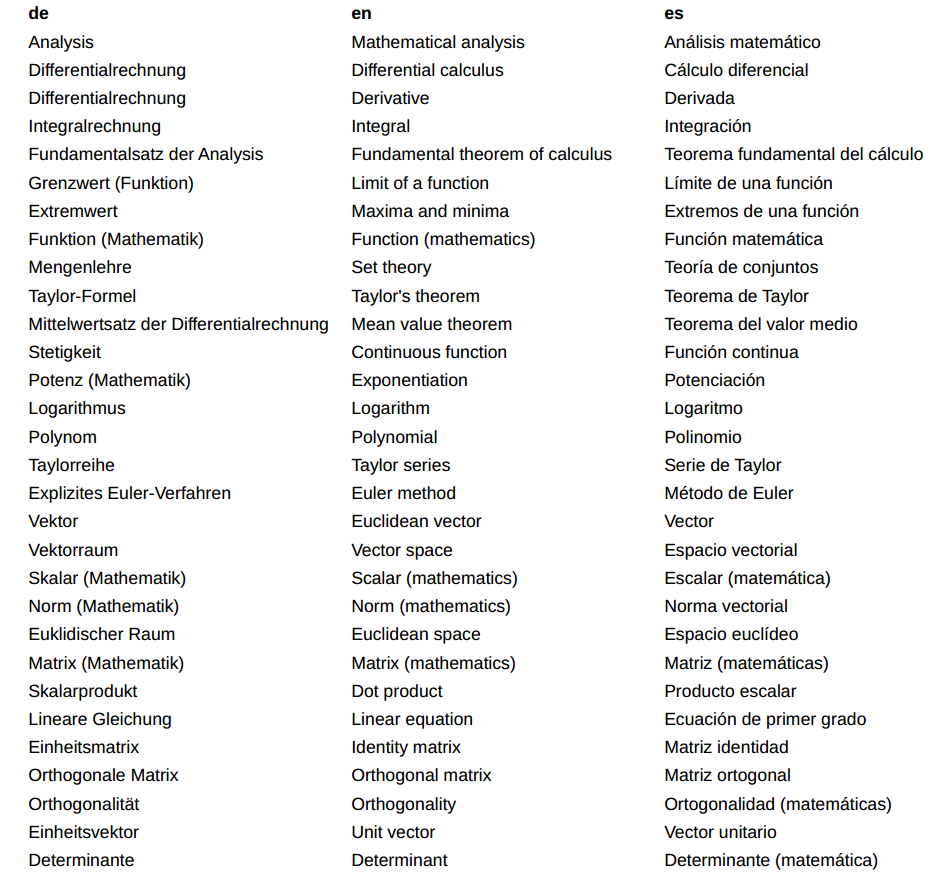
\includegraphics[scale=0.3]{mutual.png}\\
\caption{Table 1: mutual concepts, each row corresponds to a concept}
\end{center}
\subsection{Preprocessing} 
The training data is tokenized and lowercased. Stop words are removed from the data. I also tried to enforce projecting different forms of the same word into one single embedding (to make infomative words even more prominent) by stemming. But, according to the results of preliminary tests, such embeddings are harder to evaluate, so I do not include stemming in my implementation. \par
In this approach, the main objective is to make the keywords for each topic most prominent. Some POS in the corpus, like verbs, that are not stopwords and therefore are taken into account when computing embeddings, do not really fit my experiments. To enforce more interesting results, I add a POS tagger\footnote{http://www.cis.uni-muenchen.de/~schmid/tools/TreeTagger/ I intentionally do not use NLTK taggers here.} and keep only adjectives and nouns (including proper names). For Spanish, I also include past participle forms to preserve some important terms like ``derivada'' (derivative).
\section{Evaluation}
Comparing cross-lingual word embeddings is not a trivial task, especially without integrating complex NLP tasks (cannot be implemented within this project). Here I provide only a basic evaluation.
\subsection{Experiment 1}
The aim of this experiment is to project onto one concept per iteration. That is, each concept is assigned to 35 words from each language that are supposed to represent this concept (these are the word with the highest PPMI). The words \textit{across} the languages are expected to be roughly related to each other (ideally, to be translations, like ``derivative'' - ``Ableitung'' - ``derivada'' for the concept ``function''). I also expect less related topic to be represented by different words.\par
Results without filtering POS tags seem to contain much noise and are hard to interpret. Filtering helps to get better results, even if they are still far from what was expected. Smoothing does not seem to significantly influence the result. One can see the same personal names across the languages, e.g Baire, Taylor, Euler, or related terms within one concept, e.g for the concept ``dot product'': ``Kosinuswerte'' for German, $\Theta$ for English, ``cos''/``coseno'' and ``radianes'' for Spanish, or ``Gewichts'' vs. ``weights''. As expected, there are also differences between the concepts: for example, the word ``matrix'' or ``matriz'' occurs in concepts that are more related to linear algebra than to calculus. \par
I provide some files with full tables for all the concepts.
\subsection{Experiment 2}
This experiment compares words of the \textit{same} language in terms of the distance between their vectors. To measure the distance I use the \textit{cosine similarity}\cite{j} and Euclidean distance\footnote{https://en.wikipedia.org/wiki/Euclidean_distance} . The cos similarity corresponds to the cosine of the angle between two vectors: the larger the cosine value, the smaller the angle and therefore the closer the word representations. Euclidean metric captures the straight-line distance between two vectors, that means, the smaller the distance, the smaller the difference. \par
Here I expect ``similar'' words to have larger cosine values and smaller Euclidean distance. This is verified by most of the test runs. For example, in German ``Matrix'' and ``Determinante''(\textit{cos = 0.8, E.d. = 3.4}) have more similar representations than ``Funktion'' and ``Matrix''(\textit{cos = 0, E.d. = 6.4}), in English: ``function'' and ``maximum''(\textit{cos = 0.4, E.d. = 5.8}) vs ``function'' and ``matrix''(\textit{cos = 0, E.d. = 6.3}). Smoothing and POS filtering do not have a significant impact on the results.
\subsection{Experiment 3}
This experiment attempts to compare words in the same way as experiment 2, but \textit{across} the languages. In this case, I also expect larger cosine values and smaller Euclidean distance between ``related'' words, ecpecially between the translations of the same word. The results also contain shared concepts.\par
Again, my expectations are verified by the tests: ``Funktion''(de) and ``function''(en) are considered similar (\textit{cos = 0.8, E.d. = 2.4}), as well as ``Ableitung''(de) and ``derivada''(es) (\textit{cos = 0.9, E.d. = 2}). Words ``function/Funktion/funci\'on'' and ``matrix/Matrix/matriz'' have the zero cosine value since they do not have concepts in common. Here I obtain slightly better results without both smoothing and filtering or with filtering and without smoothing.
 
\subsection{Conclusion}
This simple approach allows to build an approximation of the ``multilingual MoMA semantic space'', as verified by experiments 2 and 3. With this tool users can measure the similarity between words within one language or across different languages. It also displays shared concepts for multilingual embeddings. \par 
Cross-lingual word embeddings are hard to compare (s. experiment 1), more sophisticated experiments are necessary for more informative evaluation.\par
The size and the content of corpora have a large impact on the quality of word embeddings. Wikipedia seems to be a good source for multilingual parallel corpora. \par
Laplace smoothing discounts the non-zero values, but is not crucial for the performance. Filtering POS tags is only important for experiment 1, its application and relevance should be explored more carefully.\par
\section{User Guide}
\begin{itemize}
\item to start experiments run \textit{process.py}
\item \textit{process.py} has to be in the same directory as \textit{invert.py}
\item you need internet connection to load the Wikipedia articles
\item training the embeddings takes about 1-2 minutes
\item you can choose whether to use smoothing and filtering
\item you can choose the experiment (numbers correspond to the experiments in this report)
\item you can perform experiments as long as you want :)
\end{itemize}
%----------------------------------------------------------------------------------------
%	BIBLIOGRAPHY
%----------------------------------------------------------------------------------------
 \newpage
\begin{thebibliography}{99} % Bibliography - this is intentionally simple in this template

\bibitem[S\o gaard et al.]{b}
Anders S\o gaard, Zeljko Agic, Hector Martinez Alonso, Barbara Plank, and Bernd Bohnet (2015).
\newblock Inverted indexing for cross-lingual NLP
\newblock {\em In \textit{ACL}, Vol. 1}, 1713--1722.

\bibitem[Jurafsky \& Martin]{j}
Daniel Jurafsky and James H. Martin (2017).
\newblock Speech and Language Processing.
\newblock {\em Third Edition draft}, 275--291.

 
\end{thebibliography}

%For the final project, I would like to implement the inverted indexing approach to obtain word representations. These representations can be cross-lingual and, therefore, helpful for many NLP tasks like POS-tagging, depedency parsing, word alignments, etc. I got inspired by this paper: \textit{http://www.aclweb.org/anthology/P15-1165}, which I presented in Word embeddings for NLP and IR seminar this semester.
%
%In a nutshell, each word is represented by a row in the co-occurrence  concept-word matrix. A concept is represented by some Wikipedia articles which describe the same topic in \textit{different languages} and are linked to the same node in the Wikipedia ontology.
%With the forward indexing, we would list the words per concept, but here we make use of the inverted indexing and list the concepts per word .
%
%This approach is counted-based, that means, a word is described by a vector which stores the information about how often this word is used to describe different concepts. That is, for each language, we need one co-occurrence matrix. Such matrices allow to capture relatedness between the words in different languages: words describing the same concepts have similar vectors. For example, if the German word \textit{Brille} and the English \textit{glasses} both occur in the Wiki article about Harry Potter, they will have similar representations. 
%
%The paper does not describe the approach in detail, so I think it would be challenging enough just to implement the representations. They do different experiments with these embeddings, but it would not be manageable to recreate them within 25 hours. Fortunately, they also provide the Wikipedia data here: \textit{https://sites.google.com/site/rmyeid/projects/polyglot} (which even seems to work ;)). My plan is to do the following:
%\begin{enumerate}
%\item Implement a method for constructing matrices from the given data
%\item Create matrices for some languages (preferably for the languages I speak, so I can easily evaluate my method)
%\item Compare vector representations and extract similar words (here I think of some kind of alignments: e.g., Brille and glasses are aligned together)
%\item For the evaluation, I have two ideas: 1) just automatically check whether the aligned words really have similar vectors (not sure whether this would make sense though) 2) create gold alignments manually and compare, compute recall, precision, F-score (I hope I will have time for this). 


\end{enumerate}


\end{document}